\documentclass[tikz,border=3pt]{standalone}
% Shared preamble for the standalone TikZ diagrams (included after \documentclass).
% Build with build.sh. Language is selected with \def\VI{1} (Vietnamese) or by default English:
%   \LL{English text}{Văn bản tiếng Việt}
\usepackage{fontspec}
\IfFontExistsTF{Times New Roman}{\setmainfont{Times New Roman}}{%
  \setmainfont{times.ttf}[Path=/mnt/c/Windows/Fonts/,
    BoldFont=timesbd.ttf,ItalicFont=timesi.ttf,BoldItalicFont=timesbi.ttf]}
\usepackage{xcolor}
\usepackage{tikz}
\usetikzlibrary{arrows.meta,positioning,calc,fit,backgrounds,patterns,shapes.misc,decorations.pathreplacing}

\newcommand{\LL}[2]{\ifdefined\VI #2\else #1\fi}
\hyphenpenalty=10000 \exhyphenpenalty=10000 \tolerance=9999 \emergencystretch=3em

% --- palette (print-safe: meaning is never carried by colour alone) -----------
\definecolor{ink}{HTML}{1F2937}
\definecolor{muted}{HTML}{6B7280}
\definecolor{rule}{HTML}{9CA3AF}
\definecolor{shfill}{HTML}{DCE8F5}   % shared
\definecolor{shline}{HTML}{2F5D8C}
\definecolor{dedfill}{HTML}{FBE5CF}  % dedicated
\definecolor{dedline}{HTML}{B5651D}
\definecolor{neutral}{HTML}{F3F4F6}
\definecolor{appfill}{HTML}{F6F9FC}
\definecolor{appline}{HTML}{7C93AD}
\definecolor{ctlfill}{HTML}{EFEAF7}
\definecolor{ctlline}{HTML}{6B5B95}
\definecolor{warn}{HTML}{B91C1C}
\definecolor{ta}{HTML}{2A9D8F}       % tenant A
\definecolor{tb}{HTML}{E09F3E}       % tenant B
\definecolor{tc}{HTML}{8E6BBF}       % tenant C
\colorlet{taL}{ta!22}
\colorlet{tbL}{tb!28}
\colorlet{tcL}{tc!24}

\tikzset{
  >=Latex,
  every node/.style={font=\footnotesize, text=ink, inner sep=2pt},
  box/.style={draw=ink!65, rounded corners=1.6pt, line width=0.5pt, fill=white,
              align=center, inner sep=3pt, minimum height=5mm},
  shared/.style={box, fill=shfill, draw=shline},
  ded/.style={box, fill=dedfill, draw=dedline},
  plain/.style={box, fill=neutral, draw=rule},
  ta/.style={box, fill=taL, draw=ta},
  tb/.style={box, fill=tbL, draw=tb},
  tc/.style={box, fill=tcL, draw=tc},
  tenantA/.style={ta}, tenantB/.style={tb}, tenantC/.style={tc},
  zone/.style={draw=appline, fill=appfill, rounded corners=2.5pt, line width=0.6pt},
  ctlzone/.style={draw=ctlline, fill=ctlfill, rounded corners=2.5pt, line width=0.6pt},
  ttl/.style={font=\small\bfseries, text=ink, align=left, inner sep=1pt},
  cp/.style={font=\scriptsize, text=muted, align=center, inner sep=1pt},
  note/.style={font=\scriptsize, text=muted, align=left, inner sep=1pt},
  arr/.style={->, line width=0.6pt, draw=ink!80},
  arrm/.style={->, line width=0.6pt, draw=muted, dashed},
  link/.style={line width=0.5pt, draw=muted},
  bound/.style={line width=0.8pt, draw=warn, dash pattern=on 3pt off 2pt},
  badge/.style={circle, fill=ink, text=white, font=\scriptsize\bfseries, inner sep=1.2pt, minimum size=3.6mm},
}

% a small user glyph (head + shoulders) centred at the given coordinate, colour as 3rd arg

% user glyph: head and shoulders, centred at (x,y); 3rd argument = colour
\newcommand{\user}[3]{%
  \fill[#3] (#1,#2) circle (0.85mm);
  \fill[#3] ($(#1,#2)+(-1.5mm,-2.5mm)$) arc (180:0:1.5mm) -- cycle;}

% Figure: modern multi-tenant architecture stack (improvement on Kabbedijk 2014, Fig. 2.2 / Fig. 6.2).
% Each layer lists its components and the unit at which tenants can be given a dedicated part instead of a shared one.
\begin{document}
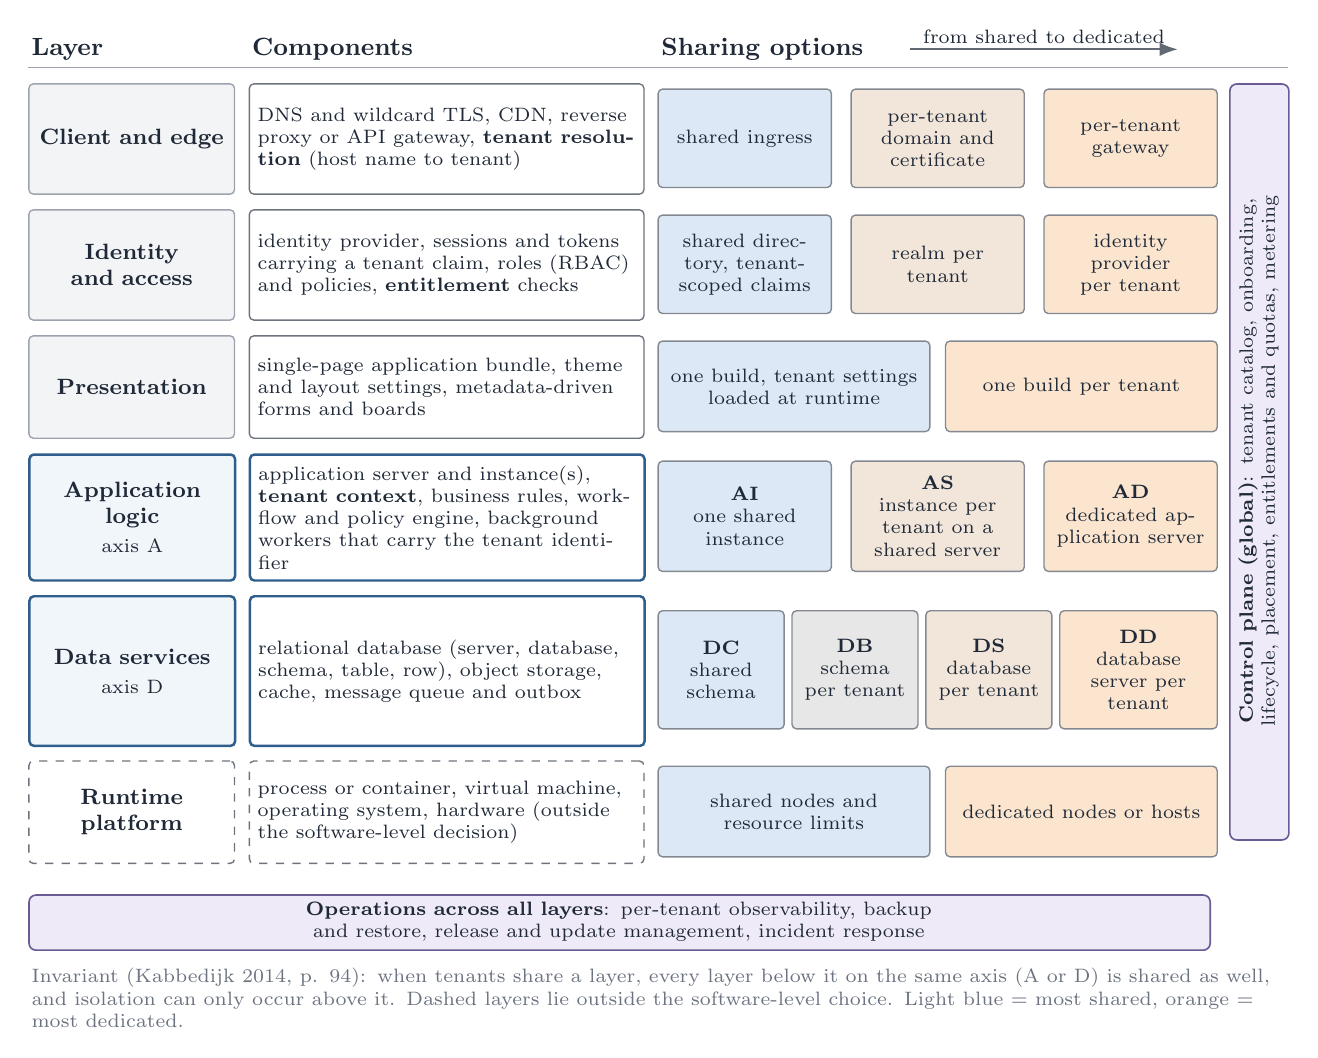
\begin{tikzpicture}[x=1mm,y=1mm]

% chip(x-left, y-centre, width, height, fill, text)
\newcommand{\chip}[6]{\node[box,fill=#5,draw=ink!55,minimum width=#3mm,minimum height=#4mm,text width=#3mm-2mm,font=\scriptsize,inner sep=1.5pt] at (#1+#3/2,#2) {#6};}
\colorlet{g1}{shfill}
\colorlet{g2}{shfill!62!dedfill}
\colorlet{g3}{shfill!30!dedfill}
\colorlet{g4}{dedfill}

% ---------------------------------------------------------------- header
\node[ttl,anchor=south west] at (0,108.5) {\LL{Layer}{Tầng}};
\node[ttl,anchor=south west] at (28,108.5) {\LL{Components}{Thành phần}};
\node[ttl,anchor=south west] at (80,108.5) {\LL{Sharing options}{Mức chia sẻ}};
\draw[->,line width=0.8pt,draw=ink!70] (112,110.3) -- node[above=0.2mm,note,text=ink] {\LL{from shared to dedicated}{từ dùng chung đến dùng riêng}} (146,110.3);
\draw[rule,line width=0.4pt] (0,108) -- (160,108);

% ---------------------------------------------------------------- rows
% L6 client and edge
\node[plain,minimum width=26mm,minimum height=14mm,text width=24mm,anchor=north west] at (0,106) {\textbf{\LL{Client and edge}{Máy khách và biên}}};
\node[box,minimum width=50mm,minimum height=14mm,text width=48mm,align=left,anchor=north west,font=\scriptsize] at (28,106) {\LL{DNS and wildcard TLS, CDN, reverse proxy or API gateway, \textbf{tenant resolution} (host name to tenant)}{DNS và TLS ký tự đại diện, CDN, proxy ngược hoặc API gateway, \textbf{nhận diện thuê bao} (tên miền tới thuê bao)}};
\chip{80}{99}{22}{12.5}{g1}{\LL{shared ingress}{lối vào dùng chung}}
\chip{104.5}{99}{22}{12.5}{g3}{\LL{per-tenant domain and certificate}{tên miền và chứng chỉ riêng}}
\chip{129}{99}{22}{12.5}{g4}{\LL{per-tenant gateway}{gateway riêng}}

% L5 identity and access
\node[plain,minimum width=26mm,minimum height=14mm,text width=24mm,anchor=north west] at (0,90) {\textbf{\LL{Identity and access}{Định danh và truy cập}}};
\node[box,minimum width=50mm,minimum height=14mm,text width=48mm,align=left,anchor=north west,font=\scriptsize] at (28,90) {\LL{identity provider, sessions and tokens carrying a tenant claim, roles (RBAC) and policies, \textbf{entitlement} checks}{nhà cung cấp danh tính, phiên và mã xác thực mang định danh thuê bao, vai trò (RBAC) và chính sách, kiểm tra \textbf{quyền sử dụng}}};
\chip{80}{83}{22}{12.5}{g1}{\LL{shared directory, tenant-scoped claims}{thư mục dùng chung, định danh thuê bao trong token}}
\chip{104.5}{83}{22}{12.5}{g3}{\LL{realm per tenant}{vùng định danh riêng}}
\chip{129}{83}{22}{12.5}{g4}{\LL{identity provider per tenant}{nhà cung cấp danh tính riêng}}

% L4 presentation
\node[plain,minimum width=26mm,minimum height=13mm,text width=24mm,anchor=north west] at (0,74) {\textbf{\LL{Presentation}{Trình diễn}}};
\node[box,minimum width=50mm,minimum height=13mm,text width=48mm,align=left,anchor=north west,font=\scriptsize] at (28,74) {\LL{single-page application bundle, theme and layout settings, metadata-driven forms and boards}{gói ứng dụng một trang, cấu hình giao diện và bố cục, biểu mẫu và bảng dựng từ siêu dữ liệu}};
\chip{80}{67.5}{34.5}{11.5}{g1}{\LL{one build, tenant settings loaded at runtime}{một bản dựng, cấu hình thuê bao nạp lúc chạy}}
\chip{116.5}{67.5}{34.5}{11.5}{g4}{\LL{one build per tenant}{mỗi thuê bao một bản dựng}}

% L3 application logic (A axis)
\node[box,fill=shfill!40,draw=shline,line width=0.9pt,minimum width=26mm,minimum height=16mm,text width=24mm,anchor=north west] at (0,59) {\textbf{\LL{Application logic}{Logic ứng dụng}}\\[1pt]{\scriptsize\LL{axis A}{trục A}}};
\node[box,draw=shline,line width=0.9pt,minimum width=50mm,minimum height=16mm,text width=48mm,align=left,anchor=north west,font=\scriptsize] at (28,59) {\LL{application server and instance(s), \textbf{tenant context}, business rules, workflow and policy engine, background workers that carry the tenant identifier}{máy chủ và thể hiện ứng dụng, \textbf{ngữ cảnh thuê bao}, quy tắc nghiệp vụ, bộ máy quy trình và chính sách, tiến trình nền mang định danh thuê bao}};
\chip{80}{51}{22}{14}{g1}{\textbf{AI}\\\LL{one shared instance}{một thể hiện dùng chung}}
\chip{104.5}{51}{22}{14}{g3}{\textbf{AS}\\\LL{instance per tenant on a shared server}{mỗi thuê bao một thể hiện trên máy chủ chung}}
\chip{129}{51}{22}{14}{g4}{\textbf{AD}\\\LL{dedicated application server}{máy chủ ứng dụng riêng}}

% L2 data services (D axis)
\node[box,fill=shfill!40,draw=shline,line width=0.9pt,minimum width=26mm,minimum height=19mm,text width=24mm,anchor=north west] at (0,41) {\textbf{\LL{Data services}{Dịch vụ dữ liệu}}\\[1pt]{\scriptsize\LL{axis D}{trục D}}};
\node[box,draw=shline,line width=0.9pt,minimum width=50mm,minimum height=19mm,text width=48mm,align=left,anchor=north west,font=\scriptsize] at (28,41) {\LL{relational database (server, database, schema, table, row), object storage, cache, message queue and outbox}{CSDL quan hệ (máy chủ, cơ sở dữ liệu, lược đồ, bảng, dòng), lưu trữ đối tượng, bộ nhớ đệm, hàng đợi thông điệp và outbox}};
\chip{80}{31.5}{16}{15}{g1}{\textbf{DC}\\\LL{shared schema}{lược đồ chung}}
\chip{97}{31.5}{16}{15}{g2}{\textbf{DB}\\\LL{schema per tenant}{lược đồ riêng}}
\chip{114}{31.5}{16}{15}{g3}{\textbf{DS}\\\LL{database per tenant}{CSDL riêng}}
\chip{131}{31.5}{20}{15}{g4}{\textbf{DD}\\\LL{database server per tenant}{máy chủ CSDL riêng}}

% L1 runtime platform (dotted, not decided at software level)
\node[box,dashed,minimum width=26mm,minimum height=13mm,text width=24mm,anchor=north west] at (0,20) {\textbf{\LL{Runtime platform}{Nền tảng thực thi}}};
\node[box,dashed,minimum width=50mm,minimum height=13mm,text width=48mm,align=left,anchor=north west,font=\scriptsize] at (28,20) {\LL{process or container, virtual machine, operating system, hardware (outside the software-level decision)}{tiến trình hoặc container, máy ảo, hệ điều hành, phần cứng (ngoài quyết định ở mức phần mềm)}};
\chip{80}{13.5}{34.5}{11.5}{g1}{\LL{shared nodes and resource limits}{nút dùng chung và giới hạn tài nguyên}}
\chip{116.5}{13.5}{34.5}{11.5}{g4}{\LL{dedicated nodes or hosts}{nút hoặc máy chủ riêng}}

% ---------------------------------------------------------------- control plane bar (right)
\node[ctlzone,minimum width=7.5mm,minimum height=96mm,anchor=north west,draw=ctlline,fill=ctlfill] at (152.5,106) {};
\node[rotate=90,font=\scriptsize,text=ink,align=center,text width=92mm] at (156.25,58) {\textbf{\LL{Control plane (global)}{Mặt phẳng điều khiển (toàn cục)}}: \LL{tenant catalog, onboarding, lifecycle, placement, entitlements and quotas, metering}{danh mục, đăng ký, vòng đời, vị trí, hạn mức, đo lường}};

% ---------------------------------------------------------------- operations bar (bottom)
\node[ctlzone,minimum width=150mm,minimum height=7mm,anchor=north west,fill=ctlfill,draw=ctlline] at (0,3) {};
\node[font=\scriptsize,text width=148mm,align=center] at (75,-0.5) {\textbf{\LL{Operations across all layers}{Vận hành xuyên suốt các tầng}}: \LL{per-tenant observability, backup and restore, release and update management, incident response}{giám sát theo thuê bao, sao lưu và khôi phục, quản lý phát hành và cập nhật, xử lý sự cố}};

% ---------------------------------------------------------------- notes
\node[note,anchor=north west,text width=158mm] at (0,-6) {\LL{Invariant (Kabbedijk 2014, p. 94): when tenants share a layer, every layer below it on the same axis (A or D) is shared as well, and isolation can only occur above it. Dashed layers lie outside the software-level choice. Light blue = most shared, orange = most dedicated.}{Nguyên lý bất biến (Kabbedijk 2014, tr. 94): khi các thuê bao dùng chung một tầng thì mọi tầng bên dưới trên cùng trục (A hoặc D) cũng dùng chung, và chỉ có thể cô lập ở các tầng phía trên. Tầng viền đứt nằm ngoài lựa chọn ở mức phần mềm. Xanh nhạt = dùng chung nhiều nhất, cam = dùng riêng nhiều nhất.}};

\end{tikzpicture}
\end{document}
